Como exemplo para a aplicação de barras de incerteza, continuaremos com os mesmo dados da seção \nameref{sec:reta}, porém agora com as incertezas associadas a cada medida, que, foram criadas, novamente, com o auxílio de um computador.


\subsection{Adicionando Colunas}

    \begin{figure}[htbp]
        \centering
        \begin{subfigure}{0.27\textwidth}
            \centering
            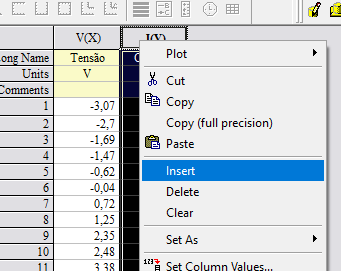
\includegraphics[width=\textwidth]{incert/1insert.png}

            \caption{Inserindo novas colunas}
            \label{fig:incert:insert}
        \end{subfigure}
        ~
        \begin{subfigure}{0.35\textwidth}
            \centering
            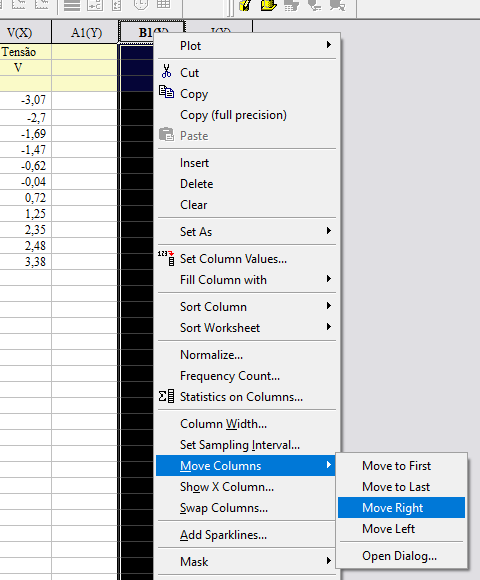
\includegraphics[width=\textwidth]{incert/2move.png}

            \caption{Mudando a posição das colunas}
            \label{fig:incert:mover}
        \end{subfigure}
        \caption{Criando novas colunas}
        \label{fig:incert:colunas}
    \end{figure}

    Para adicionar a incertezas, é preciso gerar novas colunas nas tabelas, como mostra a figura \ref{fig:incert:colunas}, lembrando sempre de formatá-las como na seção \nameref{sec:basico:renome}. A tabela com os dados de incerteza deve ficar algo parecido com a figura \ref{fig:incert:dados}.

    \begin{figure}[htbp]
        \centering
        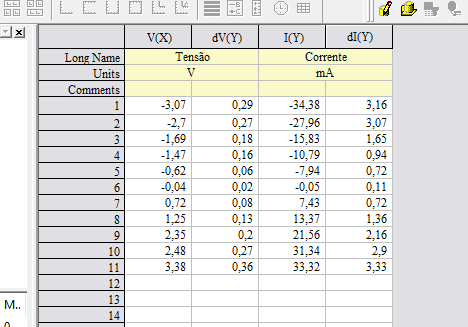
\includegraphics[width=0.7\textwidth]{incert/3dados.png}

        \caption{Dados atualizados com as incertezas}
        \label{fig:incert:dados}
    \end{figure}


\subsection{Tipo das Novas Colunas}

    \begin{figure}[htbp]
        \centering
        \begin{subfigure}{0.45\textwidth}
            \centering
            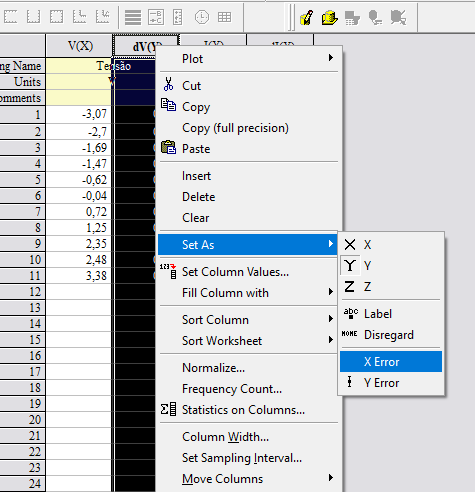
\includegraphics[width=\textwidth]{incert/4xer.png}

            \caption{Incerteza em \texttt{X}}
            \label{fig:incert:xer}
        \end{subfigure}
        ~
        \begin{subfigure}{0.45\textwidth}
            \centering
            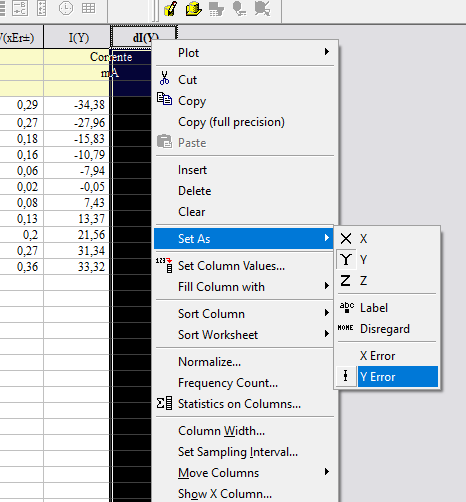
\includegraphics[width=\textwidth]{incert/5yer.png}

            \caption{Incerteza em \texttt{Y}}
            \label{fig:incert:yer}
        \end{subfigure}
        \caption{Mudando o tipo das novas colunas para relacionar com os valores das medidas}
        \label{fig:incert:tipos}
    \end{figure}


\subsection{Formatação das Barras de Incerteza}

    As barras de incerteza também têm várias configurações de formatação relacionadas a elas, mas aqui só será alterado o tamanho do traço final da barra (em inglês, \textit{cap}) como exemplo na figura \ref{fig:incert:capsz}.

    \begin{figure}[htbp]
        \centering
        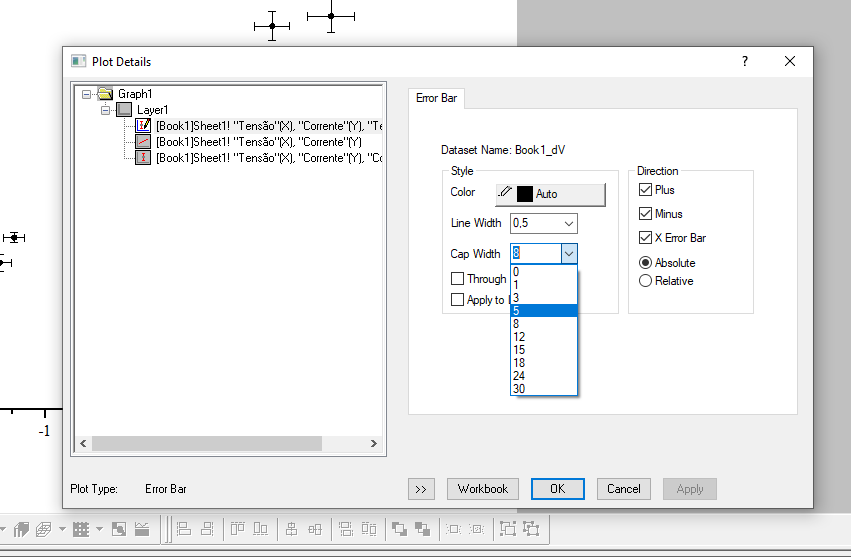
\includegraphics[width=0.7\textwidth]{incert/6cap.png}

        \caption{Dados atualizados com as incertezas}
        \label{fig:incert:capsz}
    \end{figure}


\subsection{Resultados}

    A funcionalidade \texttt{Scatter}, quando selecionada com as colunas de incerteza, gera o gráfico da figura \ref{fig:incert:preresultado}.

    \begin{figure}[htbp]
        \centering
        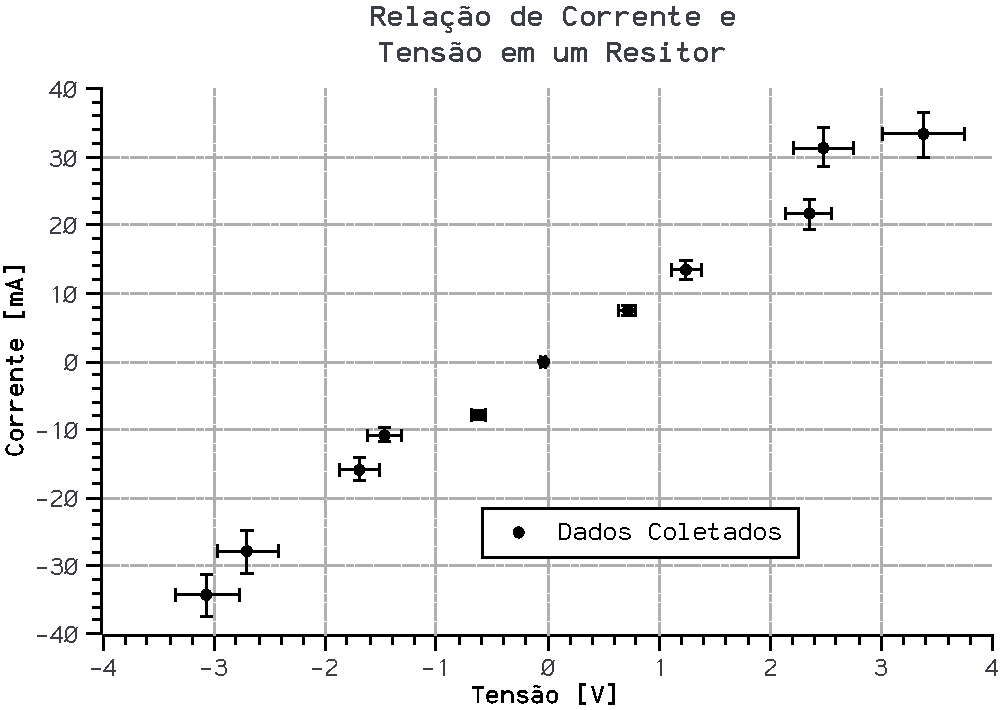
\includegraphics[width=0.8\textwidth]{incert/preresultado.pdf}

        \caption{Gráfico de corrrente por tensão com as incertezas de cada medida}
        \label{fig:incert:preresultado}
    \end{figure}

    Entretanto, se for aplicada a formatação da seção \nameref{sec:reta} e a regressão linear, como na seção \nameref{sec:regres}, o resultado deveria ficar semelhante a figura \ref{fig:incert:resultado}.

    \begin{figure}[htbp]
        \centering
        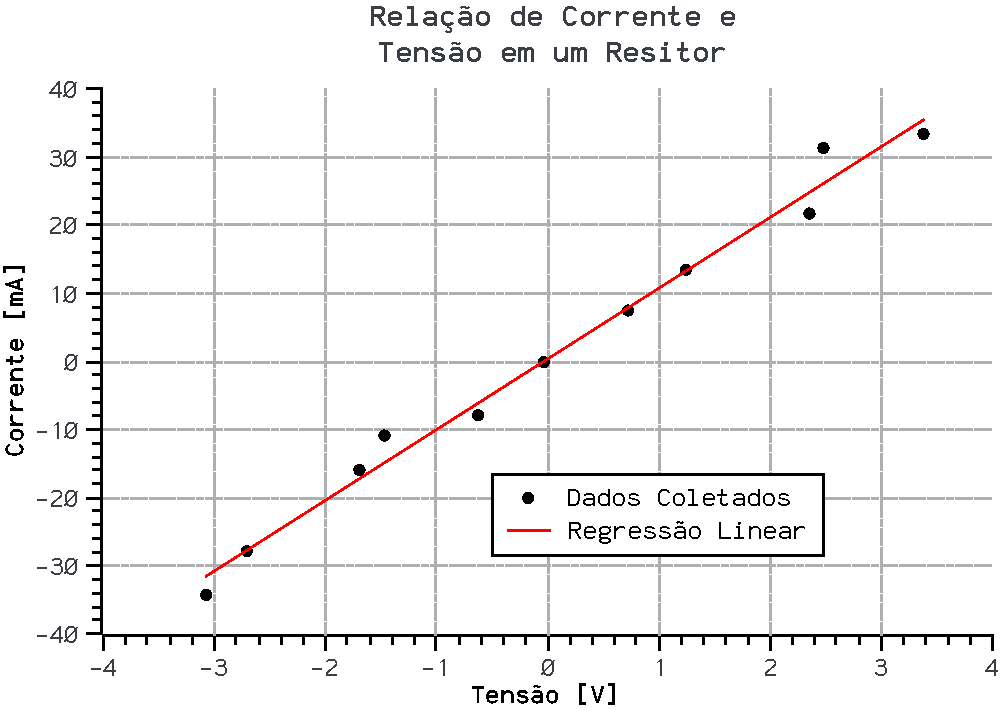
\includegraphics[width=0.8\textwidth]{incert/resultado.pdf}

        \caption{Gráfico formatado, com barras de incerteza e regressão linear}
        \label{fig:incert:resultado}
    \end{figure}

    \begin{nota}
        Note que os coeficientes da regressão em \ref{fig:incert:resultado}, tanto os valores quanto as incertezas, são levemente diferentes da figura \ref{fig:regres:final}, até mesmo com dados numéricos idênticos. A diferença aqui se deve as incertezas dos dados, que agora estão sendo levadas em conta no cálculo da regressão.

        Na verdade, apenas a incerteza em \texttt{Y} está sendo levada em conta. A regressão com as incertezas de \texttt{X} só estão presentes nas versões mais novas do \texttt{Origin}.
    \end{nota}
